\documentclass[12pt,a4paper]{article}

\usepackage[utf8]{inputenc}
\usepackage[T1]{fontenc}
\usepackage[brazilian]{babel}
\usepackage{lmodern}
\usepackage{geometry}
\usepackage{graphicx}
\usepackage{booktabs}
\usepackage{array}
\usepackage{float}
\usepackage{xcolor}
\usepackage{amsmath}
\usepackage{fancyhdr}
\usepackage{microtype}
\usepackage[hidelinks]{hyperref}

\geometry{top=2.2cm,bottom=2.2cm,left=2.4cm,right=2.4cm}
\graphicspath{{prints/}}
\pagestyle{fancy}
\fancyhf{}
\lhead{Automação Inteligente}
\rhead{Cálculos Manuais - Atividade 3A}
\cfoot{\thepage}
\setlength{\headheight}{15pt}

\begin{document}

\hypersetup{pageanchor=false}
\begin{titlepage}
  \centering
  {\large Disciplina: Automação Inteligente\par}
  \vspace{2cm}
  {\Large\bfseries ATIVIDADE PRÁTICA 3A - LÓGICA FUZZY\par}
  \vspace{0.7cm}
  {\LARGE\bfseries Cálculos Manuais Digitados em \texttt{LaTeX}\par}
  \vspace{0.8cm}
  {\Large Controle Fuzzy para Desvio de Obstáculos em Robótica Móvel\par}
  \vfill
  \begin{tabular}{rl}
    \textbf{Aluno:} & Fernando Roque Caldas de Oliveira \\
    \textbf{Matrícula:} & 202211130038 \\
    \textbf{Entradas:} & $d=10$ cm e $a=-10$ cm
  \end{tabular}
  \vfill
  {\large 2026\par}
\end{titlepage}

\hypersetup{pageanchor=true}
\pagenumbering{arabic}

\section{Dados do sistema}

As funções de pertinência especificadas na atividade são:

\begin{itemize}
  \item distância: Perto $[0,0,15,40]$, Média $[15,50,85]$ e Longe $[60,85,100,100]$;
  \item assimetria: Negativa $[-50,-50,-25,0]$, Zero $[-25,0,25]$ e Positiva $[0,25,50,50]$;
  \item saída: Virar à Esquerda $[-45,-45,-20,0]$, Seguir em Frente $[-20,0,20]$ e Virar à Direita $[0,20,45,45]$.
\end{itemize}

O sistema é Mamdani, com conectivo E pelo mínimo, implicação pelo mínimo,
agregação pelo máximo e defuzzificação pelo Centro de Área (CDA).

\section{Fase 1 - Fuzzificação das entradas}

\subsection{Distância frontal \texorpdfstring{$d=10$ cm}{d=10 cm}}

Como $10$ pertence ao patamar da função Perto, $0\leq d\leq 15$,
e está antes do suporte das funções Média e Longe:

\[
\boxed{\mu_{\text{Perto}}(10)=1{,}0},\qquad
\boxed{\mu_{\text{Média}}(10)=0{,}0},\qquad
\boxed{\mu_{\text{Longe}}(10)=0{,}0}.
\]

\subsection{Assimetria lateral \texorpdfstring{$a=-10$ cm}{a=-10 cm}}

O valor $a=-10$ pertence aos trechos lineares de Negativa e Zero. Para
Negativa, a reta decresce de $1$ em $a=-25$ para $0$ em $a=0$:

\begin{align*}
\mu_{\text{Negativa}}(-10)
&=\frac{0-a}{0-(-25)}
=\frac{0-(-10)}{25}
=\frac{10}{25}
=\boxed{0{,}4}.
\end{align*}

Para Zero, a reta cresce de $0$ em $a=-25$ para $1$ em $a=0$:

\begin{align*}
\mu_{\text{Zero}}(-10)
&=\frac{a-(-25)}{0-(-25)}
=\frac{-10+25}{25}
=\frac{15}{25}
=\boxed{0{,}6}.
\end{align*}

Como $-10<0$, a função Positiva ainda não possui suporte:

\[
\boxed{\mu_{\text{Positiva}}(-10)=0{,}0}.
\]

\begin{figure}[H]
  \centering
  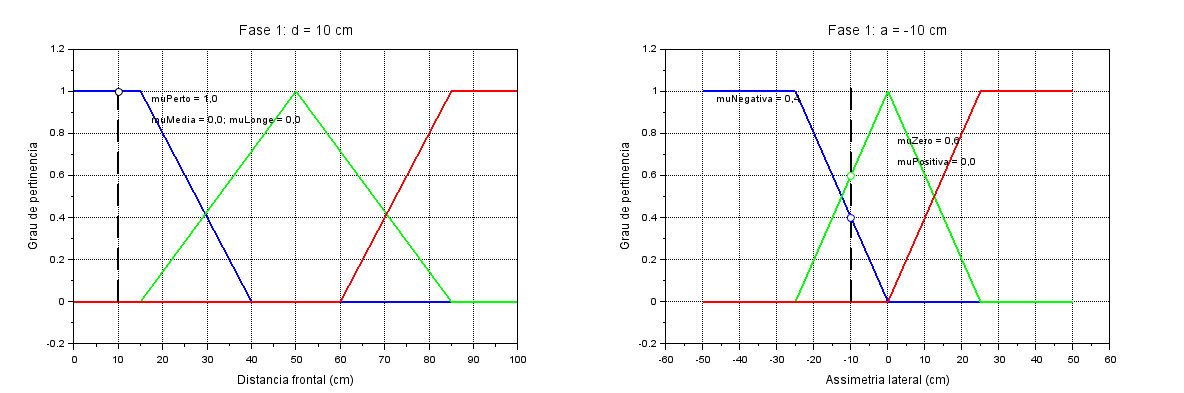
\includegraphics[width=\textwidth]{05_fase1_entradas_anotadas.png}
  \caption{Valores de entrada marcados e graus de pertinência calculados.}
\end{figure}

\section{Fase 2 - Identificação das regras ativadas}

Como somente Perto, Negativa e Zero possuem pertinência diferente de zero,
exatamente duas regras são ativadas:

\begin{enumerate}
  \item Se a distância é Perto e a assimetria é Negativa, então o ângulo é Virar à Esquerda.
  \item Se a distância é Perto e a assimetria é Zero, então o ângulo é Virar à Direita.
\end{enumerate}

\section{Fase 3 - Conectivo E e implicação de Mamdani}

As forças das regras são obtidas pelo operador mínimo:

\begin{align*}
\alpha_1
&=\min\left(\mu_{\text{Perto}}(10),\mu_{\text{Negativa}}(-10)\right)
=\min(1{,}0;0{,}4)
=\boxed{0{,}4},\\[0.4cm]
\alpha_2
&=\min\left(\mu_{\text{Perto}}(10),\mu_{\text{Zero}}(-10)\right)
=\min(1{,}0;0{,}6)
=\boxed{0{,}6}.
\end{align*}

Na implicação de Mamdani, cada consequente é truncado pela força de sua regra:

\begin{align*}
\mu_{R1}(\theta)
&=\min\left(0{,}4;\mu_{\text{Virar Esquerda}}(\theta)\right),\\
\mu_{R2}(\theta)
&=\min\left(0{,}6;\mu_{\text{Virar Direita}}(\theta)\right).
\end{align*}

\section{Fase 4 - Agregação das contribuições}

As duas saídas truncadas são combinadas ponto a ponto pelo operador máximo:

\[
\boxed{
\mu_{\text{agregada}}(\theta)
=\max\left(\mu_{R1}(\theta),\mu_{R2}(\theta)\right)
}.
\]

\begin{figure}[H]
  \centering
  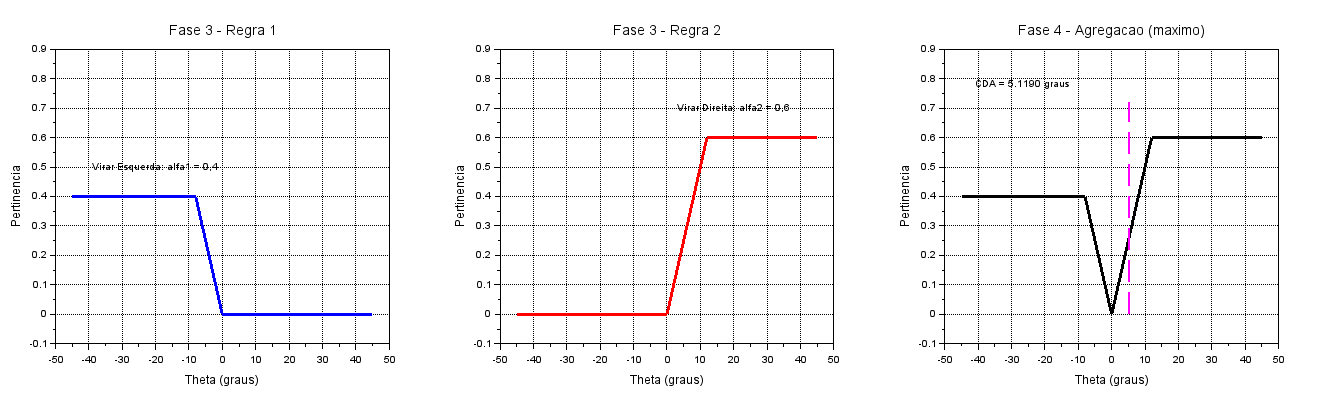
\includegraphics[width=\textwidth]{06_fases3_4_implicacao_agregacao.png}
  \caption{Implicação das duas regras e agregação pelo máximo.}
\end{figure}

\section{Fase 5 - Defuzzificação pelo Centro de Área}

O universo $[-45^\circ,45^\circ]$ é discretizado em passos de $5^\circ$.
Para cada amostra calculam-se a pertinência agregada e o produto
$\mu(\theta)\theta$.

\begin{table}[H]
\centering
\caption{Tabela completa do cálculo manual do CDA.}
\setlength{\tabcolsep}{10pt}
\begin{tabular}{rrr@{\qquad}rrr}
\toprule
$\theta$ & $\mu(\theta)$ & $\mu(\theta)\theta$ &
$\theta$ & $\mu(\theta)$ & $\mu(\theta)\theta$ \\
\midrule
-45 & 0,40 & -18,00 & 5  & 0,25 & 1,25 \\
-40 & 0,40 & -16,00 & 10 & 0,50 & 5,00 \\
-35 & 0,40 & -14,00 & 15 & 0,60 & 9,00 \\
-30 & 0,40 & -12,00 & 20 & 0,60 & 12,00 \\
-25 & 0,40 & -10,00 & 25 & 0,60 & 15,00 \\
-20 & 0,40 & -8,00  & 30 & 0,60 & 18,00 \\
-15 & 0,40 & -6,00  & 35 & 0,60 & 21,00 \\
-10 & 0,40 & -4,00  & 40 & 0,60 & 24,00 \\
-5  & 0,25 & -1,25  & 45 & 0,60 & 27,00 \\
0   & 0,00 & 0,00   &    &      &       \\
\bottomrule
\end{tabular}
\end{table}

\subsection*{Memorial do denominador}

No lado esquerdo há oito amostras com pertinência $0{,}40$ e uma com
$0{,}25$. No lado direito há $0{,}25$, $0{,}50$ e sete amostras com
$0{,}60$:

\begin{align*}
\sum\mu(\theta)
&=(8\cdot0{,}40+0{,}25)+(0{,}25+0{,}50+7\cdot0{,}60)\\
&=3{,}45+4{,}95\\
&=\boxed{8{,}40}.
\end{align*}

\subsection*{Memorial do numerador}

\begin{align*}
\sum\mu(\theta)\theta
&=0{,}40(-45-40-35-30-25-20-15-10)+0{,}25(-5)\\
&\quad+0{,}25(5)+0{,}50(10)
+0{,}60(15+20+25+30+35+40+45)\\
&=-89{,}25+132{,}25\\
&=\boxed{43{,}00}.
\end{align*}

\subsection*{Cálculo final do CDA}

\begin{align*}
\theta_{\text{manual}}
&=\frac{\sum\mu(\theta)\theta}{\sum\mu(\theta)}
=\frac{43{,}00}{8{,}40}
=\boxed{5{,}119048^\circ}.
\end{align*}

Como o ângulo é positivo, a ação final é:

\[
\boxed{\text{VIRAR PARA A DIREITA}}.
\]

\section{Comparação com a simulação}

\begin{table}[H]
\centering
\caption{Comparação entre o cálculo manual e o Scilab.}
\renewcommand{\arraystretch}{1.3}
\begin{tabular}{lcc}
\toprule
\textbf{Método} & \textbf{Ângulo} & \textbf{Decisão} \\
\midrule
Cálculo manual, passo de $5^\circ$ & $5{,}119048^\circ$ & Virar à direita \\
Simulação Scilab/sciFLT, 1001 pontos & $4{,}828622^\circ$ & Virar à direita \\
Diferença (simulado $-$ manual) & $-0{,}290426^\circ$ & Mesma decisão \\
\bottomrule
\end{tabular}
\end{table}

A pequena diferença decorre exclusivamente da resolução de discretização.
Os dois métodos produzem ângulo positivo e indicam a mesma ação de controle.

\end{document}
